\documentclass[aoas,preprint]{imsart}

\RequirePackage[OT1]{fontenc}
\RequirePackage{amsthm,amsmath}
\RequirePackage[numbers]{natbib}
\RequirePackage[colorlinks,citecolor=blue,urlcolor=blue]{hyperref}

\usepackage{graphicx}
\usepackage{algorithm}
\usepackage{algpseudocode}

\usepackage{amssymb,amsmath,amsthm,amsfonts}
\usepackage{mathrsfs}
\usepackage{dsfont}
\usepackage{enumerate}

%\newtheorem{mdef}{Definition}
%\newtheorem{theorem}{Theorem}
\newcommand{\eqsplit}[2]{
  \begin{equation}\label{#2}
    \begin{split}
      #1
    \end{split}
  \end{equation}}
\newcommand{\eqnsplit}[1]{
  \begin{eqnarray*}
    #1
  \end{eqnarray*}}
\newcommand{\tran}[1]{
  \tilde{#1}
}
\newcommand{\td}[2]{
  \frac{d #1}{d #2}
}
\newcommand{\pd}[2]{
  \frac{\partial #1}{\partial #2}
}
\newcommand{\ppd}[2]{
  \frac{\partial^2 #1}{\partial #2^2}
}
\newcommand{\pdd}[3]{
  \frac{\partial^2 #1}{\partial #2 \partial #3}
}
\newcommand{\otd}[1]{
  \frac{d}{d #1}
}
\newcommand{\opd}[1]{
  \frac{\partial}{\partial #1}
}
\newcommand{\oppd}[1]{
  \frac{\partial^2}{\partial #1^2}
}
\newcommand{\opdd}[2]{
  \frac{\partial^2}{\partial #1 \partial #2}
}
\newcommand{\ket}[1]{
  |#1\rangle
}
\newcommand{\bra}[1]{
  \langle#1|
}
\newcommand{\inn}[1]{
  \langle#1\rangle
}
\newcommand{\mean}[1]{
  \langle#1\rangle
}
\newcommand{\tr}{
  \text{tr}\,
}
\newcommand{\re}{
  \text{Re}\,
}
\newcommand\im{
  \text{Im}\,
}
\newcommand{\var}{
  \text{var}
}
\newcommand{\arcsinh}{
  \sinh^{-1}
}
\newcommand{\arccosh}{
  \cosh^{-1}
}
\newcommand{\erfc}{
  \text{erfc}
}
\newcommand{\E}{
  \mathbb{E}
}
\renewcommand{\P}{
  \mathbb{P}
}
\newcommand{\I}[1]{
  \mathbf{1}_{\{#1\}}
}
\newcommand{\1}[1]{
  \mathds{1}_{\{#1\}}
}
\newcommand{\diag}{
  \text{diag\,}
}
\newcommand{\M}{
  {\text{max}}
}
\newcommand{\m}{
  {\text{min}}
}
\newcommand{\ph}{
  {\text{arg}\,}
}
\newcommand\erf{
  \text{erf}
}
\renewcommand\vec[1]{
  \mathbf{#1}
}
\newcommand\mtx[1]{
  \mathbf{#1}
}
\newcommand\ed{
  \,{\buildrel d \over =}\,
}




% settings
%\pubyear{2005}
%\volume{0}
%\issue{0}
%\firstpage{1}
%\lastpage{8}
\arxiv{arXiv:0000.0000}

\startlocaldefs
\numberwithin{equation}{section}
\theoremstyle{plain}
\newtheorem{thm}{Theorem}[section]
\endlocaldefs

\begin{document}

\begin{frontmatter}
\title{An importance sampling estimator of probabilities of high
  threshold exceedance by GARCH(p,q) processes\thanksref{T1}}
\runtitle{An importance sampling estimator of probabilities of high
  threshold exceedance by multivariate Markov Chains}
\thankstext{T1}{Footnote to the title with the ``thankstext'' command.}

\begin{aug}
\author{\fnms{First} \snm{Author}\thanksref{t1,t2,m1}\ead[label=e1]{first@somewhere.com}},
\author{\fnms{Second} \snm{Author}\thanksref{t3,m1,m2}\ead[label=e2]{second@somewhere.com}}
\and
\author{\fnms{Third} \snm{Author}\thanksref{t1,m2}
\ead[label=e3]{third@somewhere.com}
\ead[label=u1,url]{http://www.foo.com}}

\thankstext{t1}{Some comment}
\thankstext{t2}{First supporter of the project}
\thankstext{t3}{Second supporter of the project}
\runauthor{F. Author et al.}

\affiliation{Copenhagen University\thanksmark{m1} and Another University\thanksmark{m2}}

\address{Address of the First and Second authors\\
Usually a few lines long\\
\printead{e1}\\
\phantom{E-mail:\ }\printead*{e2}}

\address{Address of the Third author\\
Usually a few lines long\\
Usually a few lines long\\
\printead{e3}\\
\printead{u1}}
\end{aug}

\begin{abstract}
The abstract should summarize the contents of the paper.
It should be clear, descriptive, self-explanatory and not longer
than 200 words. It should also be suitable for publication in
abstracting services. Please avoid using math formulas as much as possible.

This is a sample input file.  Comparing it with the output it
generates can show you how to produce a simple document of
your own.
\end{abstract}

\begin{keyword}[class=MSC]
\kwd[Primary ]{60K35}
\kwd{60K35}
\kwd[; secondary ]{60K35}
\end{keyword}

\begin{keyword}
\kwd{sample}
\kwd{\LaTeXe}
\end{keyword}

\end{frontmatter}

\section{Introduction}
Ever since its proposition by Bollerslev~\cite{bollerslev:1986} and
Taylor~\cite{taylor:2008} (cf. also
\cite{andersen:davis:kreiss:mikosch:2009}), the GARCH
({\em Generalized Autoregressive Conditional Heteroscedasticity}) model
has seen wide-spread application in finance and economics, and has
inspired numerous variants such as GJR-GARCH of Glosten et
al~\cite{glosten:1993}, {\em Asymetric} GARCH of Engle and
Ng~\cite{engle:Ng:1993} and the {\em Quadratic} GARCH of
Sentana~\cite{sentana:1995}, among others. The basic GARCH model of
Bollerslev~\cite{bollerslev:1986} and Taylor~\cite{taylor:2008}
defines the conditional variance via the stochastic recurrence
equation
\begin{eqnarray}
  R_t &=& \sigma_t Z_t \nonumber \\
  \sigma_{t}^2 &=& \omega + \sum_{i=1}^p \alpha_i R_{t-i}^2 + \sum_{j=1}^q
  \beta_j \sigma_{t-j}^2   \label{eq:garchpq}
\end{eqnarray}
where $\{R_t\}_{t \in \mathbb Z}$ is the return series in question;
$\{Z_t\}_{t \in \mathbb Z}$ is an iid sequence of random variables
with zero mean and unit variance.
$\omega, \alpha_i, i \in \{1,\dots,p\}$ and
$\beta_j, j \in \{1,\dots,q\}$
are constant parameters. A process defined by
\eqref{eq:garchpq} is called a GARCH($p,q$) process.
Note that \eqref{eq:garchpq} can be written as a stochastic recurrence 
equation. When $p = q = 1$,
\[
\sigma_t^2 = \omega + (\alpha_1 Z_{t-1}^2 + \beta_1) \sigma_{t-1}^2
\]
When $p > 1$ or $q > 1$, a matrix recurrence equation arises
(cf. Davis and Mikosch~\cite{davis:mikosch:2001})
\begin{small}
  \begin{equation*}
    \underbrace{
      \begin{pmatrix}
        \sigma_{t}^2 \\
        \sigma_{t-1}^2 \\
        \vdots \\
        \sigma_{t-q+2}^2 \\
        \sigma_{t-q+1}^2 \\
        R_{t-1}^2 \\
        R_{t-2}^2 \\
        \vdots \\
        R_{t-p+2}^2 \\
        R_{t-p+1}^2
      \end{pmatrix}}_{V_t} =
    \underbrace{
      \begin{pmatrix}
        \alpha_1 Z_{t-1}^2 + \beta_1 & \beta_2 & \cdots &
        \beta_{q-1} & \beta_q & \alpha_2 & \alpha_3 & \cdots & \alpha_p & 0 \\
        1 & 0 & \cdots & 
        0 & 0 & 0 & 0 & \cdots & 0 & 0 \\
        \vdots & \vdots & \ddots & 
        \vdots & \vdots & \vdots & \vdots & \ddots & \vdots & \vdots \\
        0 & 0 & \cdots &
        0 & 0 & 0 & 0 & \cdots & 0 & 0 \\
        0 & 0 & \cdots &
        1 & 0 & 0 & 0 & \cdots & 0 & 0 \\
        Z_{t-1}^2 & 0 & \cdots &
        0 & 0 & 0 & 0 & \cdots & 0 & 0 \\
        0 & 0 & \cdots &
        0 & 0 & 1 & 0 & \cdots & 0 & 0 \\
        \vdots & \vdots & \ddots &
        \vdots & \vdots & \vdots & \vdots & \ddots & \vdots & \vdots \\
        0 & 0 & \cdots &
        0 & 0 & 0 & 0 & \cdots & 0 & 0 \\    
        0 & 0 & \cdots &
        0 & 0 & 0 & 0 & \cdots & 1 & 0 \\    
      \end{pmatrix}
    }_{A_t}
    \underbrace{
      \begin{pmatrix}
        \sigma_{t-1}^2 \\
        \sigma_{t-2}^2 \\
        \vdots \\
        \sigma_{t-q+1}^2 \\
        \sigma_{t-q}^2 \\
        R_{t-2}^2 \\
        R_{t-3}^2 \\
        \vdots \\
        R_{t-p+1}^2 \\
        R_{t-p}^2
      \end{pmatrix}
    }_{V_{t-1}} +
    \underbrace{
      \begin{pmatrix}
        \omega \\
        0 \\
        \vdots \\
        0 \\
        0 \\
        0 \\
        0 \\
        \vdots \\
        0 \\
        0 \\
      \end{pmatrix}
    }_{B_t}
  \end{equation*}
\end{small}
For convenience, we shall write the above recurrence equation as
\[
V_t = A_t V_{t-1} + B_t
\]
with $V_t$, $A_t$ and $B_t$ defined as above. Using the Kesten and
Goldie theorem \cite{kesten:1973}, Bollerslev showed that the
equations \eqref{eq:garchpq} has a unique, strictly stationary
solution if and only if
\[
\sum_{i=1}^p \alpha_i + \sum_{j=1}^q \beta_j < 1
\]
Cf. Buraczewski et al \cite{buraczewski:damek:mikosch:2016}.

\section{Statement of the Problem}

We are interested in developing an estimator for the probability
$\P(|V| > u)$ where the vector $V$ has the stationary
distribution of the Markov chain $V_{n} = A_n V_{n-1} + B_n$. Here
$A_n$ are i.i.d $d \times d$ random matrices and $B_n$ are
$d$-dimensional random vectors. Let $\mu$ denote the distribution of
$A_n$ and $A \sim \mu$.
\begin{enumerate}[(i)]
\item For each and every $n \geq 1$ and for all
  $1 \leq i \leq j \leq d$, $(A_n)_{i,j} > 0$.
\item With probability 1, the matrices $A_n$ have no all-zero rows or
  columns, i.e.
  \[
  \P \left\{
  \text{$\exists 1 \leq i \leq n$ such that
    $\forall 1 \leq j \leq n$, $(A_n)_{i,j} = 0$ or $(A_n)_{j,i} = 0$
  }
  \right\} = 0
  \]
  %% That is, $\mu$- almost surely $A_n$ has no zero-rows or
  %% zero-columns.
\item The additive subgroup of $\mathbb R$ generated by
  \[
  \{\ln \rho(\pi): \pi = \prod_{i=1}^n A_i \quad \text{for some n
    and iid. } A_i\}.
  \]
  is dense in $\mathbb R$. Here $\rho(\pi)$ denotes the largest
  singular value of $\pi$.
\item $\exists \xi > 0$ such that $\lambda(\xi) = 1$, where
  \[
  \lambda(\xi) := \inf_{n \geq 1} (\E \|A_n \cdots A_1\|^\xi)^{1/n}
  \]
  In addition,
  \begin{eqnarray*}
    \E \left[
      \|A\|^\xi \max\left\{
      \left| \ln(\|A\|) \right|,
      \left|
      \ln\left(\inf_{x \in S^{d-1}} |A x|\right) \right|
      \right\}
      \right] &<& \infty,
    \quad
    \E(|B|^\xi) < \infty
  \end{eqnarray*}
\item Let $\pi$ denote the stationary distribution of $V_n$ and $P$
  denote the transition kernel of $V_n$. Assume that
  there exists a set $\mathcal C$ with $\pi(\mathcal C) > 0$
  such that $\forall x \in \mathcal C$, $P(x, \cdot)$ has an
  absolutely continuous component with respect to some $\sigma$-finite
  non-null measure $\phi$.
\end{enumerate}
These are the same conditions that Collamore and
Mentemeier~\cite{collamore2016large} assumed in their hypotheses
$H_1, H_2, H_3$. One can compare them with conditions (M) and (A) of
Kesten~\cite{kesten:1973}. Under these conditions, Collamore and
mentemeier \cite{collamore2016large} showed that the chain $V_n$ is an
aperiodic, positive Harris chain on $\mathbb R_+^d$. Cf. their lemma
3.4. Moreover, it follows from condition (v)
\[
P(x, A) \geq \I_{\mathcal C}(x) \phi(A) \inf_{y \in A} f(y)
\]
where $f(\cdot)$ is the Radon-Nikodym derivative of $P(x, \cdot)$ with
respect to $\phi$. This minorization condition gives rise to a
regenerative structure of the path of $V_n$. Cf. Ney and Nummelin
\cite{ney1987markov}, lemma 3.1. Let $\tau$ has the distribution of
the length of a regeneration cycle in this structure.

For a general vector $x$, let $\tilde x$ denote ${x \over |x|}$. For
convenience, we also use the following notations:
\begin{eqnarray*}
X_n &=& {
        A_n A_{n-1} \cdots A_1 \tilde V_0
        \over
        |A_n A_{n-1} \cdots A_1 \tilde V_0|
        } \\
S_n &=& \ln |A_n \cdots A_1 \tilde V_0| \\
\xi_n &=& S_n - S_{n-1} \\
&=& \frac{|A_n \cdots A_1 \tilde V_0|}{|A_{n-1} \cdots A_1 \tilde V_0|} \\
&=& \ln\left| A_n \frac{A_{n-1} \cdots A_1 \tilde V_0}
    {|A_{n-1} \cdots A_1 \tilde V_0|} \right|\\
&=& \ln |A_n X_{n-1}|
\end{eqnarray*}
Furthermore, we define
\begin{eqnarray*}
R_n &:=& \inf\{0 \leq i \leq n: V_i \in \mathcal C\} \\
K_0 &:=& 0 \\
K_i &:=& \inf\{k \geq 1: k > K_{i-1}, V_k \in \mathcal C, K_0 = 0\} \\
N_u &:=& \sum_{i=1}^\tau \1{V_i > u} \\
T_u &=& \inf\{n \geq 1: |V_n| > u\}
\end{eqnarray*}

% \begin{theorem}
%   The pair $(X_n, S_n)$ is a Markov additive process with transition
%   kernel $P$. In addition, $(X_n, S_n)$ is Harris recurrent.
  
% \end{theorem}

\section{Consistency}\label{sec:consistency}
\begin{theorem}
  \begin{eqnarray*}
    \P(|V| > u) &=& \pi(\mathcal C) \E_{\mathcal D} \left[
      N_u \1{T_u < \tau} e^{-\xi S_{T_u}} {r(\tilde V_0; \xi)
        \over r(x_{T_u}; \xi)}
    \right]
  \end{eqnarray*}
\end{theorem}
\begin{proof}
  By the law of large numbers
  \begin{eqnarray*}
    && \P(|V| > u) \\
    &=& \lim_{n \to \infty} {1 \over n} \sum_{i=0}^n \1{|V_i| > u}
  \end{eqnarray*}
  Then one can write
  \begin{eqnarray*}
    && \lim_{n \to \infty} {1 \over n} \sum_{i=1}^n \1{|V_i| > u} \\
    &=& \lim_{n \to \infty} {1 \over n} \left[
      \sum_{i=0}^{K_{R_n}-1} \1{|V_i| > u} + \sum_{i=K_{R_n}}^n \1{|V_i| > u}
    \right]
  \end{eqnarray*}
  For the 2nd term, by a Borel-Cantelli argument, it maybe shown
  \[
  \lim_{n \to \infty} {1 \over n}\sum_{i=K_{R_n}}^n \1{|V_i| > u} = 0
  \]
  For the 1st term,
  \begin{eqnarray*}
    && \lim_{n \to \infty} {1 \over n} \sum_{i=0}^{K_{R_n}-1} \1{|V_i| >
      u}  \\
    &=& \lim_{n \to \infty} {R_n \over n} {1 \over R_n} \sum_{i=1}^{R_n}
    \sum_{j=K_{i-1}}^{K_i-1}\1{|V_i| > u} \\
    &=& \pi(\mathcal C) \E_\gamma N_u
  \end{eqnarray*}
  where the law of large numbers of Markov chains has been used to reach
  the last line. In addition, it is assumed
  \begin{eqnarray*}
    V_{K_i} &\sim& \gamma \; \forall i \geq 0 \\
    \gamma(E) &=& \pi(E)/\pi(\mathcal C)\; \forall E \in \mathcal
    B(\mathcal C)
  \end{eqnarray*}
  Then $\E_\gamma N_u$ may be evaluated as
  \begin{eqnarray*}
    && \E_\gamma N_u \\
    &=& \E_\gamma N_u \1{T_u < \tau} \\
    &=& \int_{\mathds S^{d-1}} \int_{\mathds R} \cdots \int_{\mathds
      S^{d-1}} \int_{\mathds R} N_u \1{T_u < \tau} \times \\
    && \prod_{i=1}^{T_u} e^{-\xi(s_i - s_{i-1}) + \lambda(\xi)}
    {r(x_{i-1}; \xi) \over r(x_{i}; \xi)}P_\xi(x_{i-1}, dx_i \times ds_i) \times \\
    && \prod_{i=T_u+1}^{\tau-1} P(x_{i-1}, dx_i \times d s_i) \\
    &=& \E_{\mathcal D} \left[
      N_u \1{T_u < \tau} e^{-\xi S_{T_u}} {r(\tilde V_0; \xi)
        \over r(x_{T_u}; \xi)}
    \right]
  \end{eqnarray*}
  where
  \[
  P_\xi(x_{i-1}, dx_i \times ds_i) = e^{\xi(s_i - s_{i-1}) -
    \lambda(\xi)} {r(x_i; \xi) \over r(x_{i-1}; \xi)} P(x_{i-1}, dx_i
  \times ds_i)
  \]
  is the $\xi$-shifted transition kernel of the {\it Markov Additive
    process} $(X_n, S_n)$. $\xi$ is chosen such that 
  \[
  \lambda(\xi) = \lim_{n \to \infty} \ln \left(
    \E \|A_n \cdots A_1\|^\xi
  \right)^{1/n} = 0
  \]
  $\E_{\mathcal D}$ denotes expectation taken with respect to the dual
  measure defined as
  \[
  P_{\mathcal D} (x_i, dx_{i+1} \times ds) = \left\{
    \begin{array}{ll}
      P_\xi (x_i, dx_{i+1} \times ds) & \text{ if } i < T_u \\
      P(x_i, dx_{i+1} \times ds) & \text{ if } i \geq T_u \\
    \end{array}
  \right.
  \]
  Because the top Lyapunov exponent is negative, it follows from a lemma
  in Kesten \cite{kesten:1973} that there is a $s > 0$ such that
  $\lambda(s) < 0$.

  Thus we have obtained a consistent estimator
  $\pi(\mathcal C)\mathcal E_u$ for $\P(|V| > u)$:
  \begin{eqnarray*}
    \P(|V| > u) &=& \pi(\mathcal C) \E_{\mathcal D} \left[
      N_u \1{T_u < \tau} e^{-\xi S_{T_u}} {r(\tilde V_0; \xi)
        \over r(x_{T_u}; \xi)}
    \right]
  \end{eqnarray*}
\end{proof}

\section{Efficiency}\label{sec:efficiency}
\begin{lemma}
  Let $\beta \in \mathbb R$ satisfy
  \begin{enumerate}
  \item
    \begin{equation}
      \label{eq:drift_cond1}
      \E \|A\|^\beta < \infty      
    \end{equation}
  \item 
    \begin{equation}
      \label{eq:drift_cond2}
    \inf_{\alpha > 0} {\E \|A\|^{\alpha + \beta}
      \over 
      \E \|A\|^{\beta}
    } < 1
    \end{equation}
  \end{enumerate}
  then $\forall \alpha > 0$ such that $\frac{\E\|A\|^{\beta +
      \alpha}}{\E\|A\|^\beta} < 1$ , we have
  \begin{equation}
    \label{eq:drift}
    \E_\beta \left[\left.
        |V_n|^\alpha r_\beta(|\tilde V_n|; \alpha) \I_{{\mathcal C}^\complement}(V_{n-1}) \right|
      \mathcal F_{n-1} \right] \leq |V_{n-1}|^\alpha r_\beta(|\tilde
    V_{n-1}|; \alpha) \I_{{\mathcal C}^\complement}(V_{n-1})
  \end{equation}
  where $r_\beta(\cdot; \alpha)$ is the unique right eigen function of the
  operator
  \[
  P_{\beta, \alpha} f(x) = \int |\mathbf a x|^\alpha f\left(
    {\mathbf a x \over |\mathbf a x|}
  \right) d\mu_A^\beta(\mathbf a)
  \]
  where the $\beta$-shifted measure $\mu_A^\beta$ satisfies
  \[
  d\mu_A^\beta(\mathbf a) = {\|\mathbf a\|^\beta d\mu_A(\mathbf a) \over \E\|A\|^\beta}
  \]
  The set $\mathcal C = [-M_\beta(\alpha),
  M_\beta(\alpha)]$. $M_\beta(\alpha)$ is chosen with respect to the
  values of $\alpha$ and $\beta$.
\end{lemma}

\begin{proof}
  Conditions \eqref{eq:drift_cond1} and \eqref{eq:drift_cond2} imply $\E_\beta
  \|A\|^\alpha < \infty$. Then, using the results of Buraczewski and
  Collamore et al \cite{BCDZ2014}, one may conclude that an eigen
  function $r_\beta(\cdot; \alpha)$ as well as an eigen measure
  $l_\beta(\cdot; \alpha)$ exists under the $\beta$-shifted
  measure. Thus, by defining the adjoint operator under  the shifted
  measure, the right eigen function $r_\beta(x; \alpha)$ can be represented as
  \[
  r_\beta(x; \alpha) = c \int_{S_+^{d-1}} \inn{x, y}^\alpha
  dl^*_{\beta}(y; \alpha)
  \]
Now, to prove \eqref{eq:drift}, consider
  \begin{eqnarray}
    && \E_\beta \left[ |V_n|^\alpha r_\beta(\tilde V_n; \alpha) | \mathcal F_{n-1} \right]
    \nonumber \\
    &=& \E_\beta\left[\int_{S_+^{d-1}} \inn{V_n, y}^\alpha dl^*_{\beta}(y; \alpha)|
      \mathcal F_{n-1} \right]
    \nonumber \\
    &=& \E_\beta\left[\int_{S_+^{d-1}} (\inn{A_n V_{n-1}, y} + \inn{B_n,
        y})^\alpha dl^*_{\beta}(y; \alpha) | \mathcal F_{n-1} \right]
    \label{eq:drift_proof_1}
  \end{eqnarray}
  \begin{enumerate}
  \item if $\alpha \leq 1$, by subadditivity we have
    \begin{eqnarray*}
      &&\E_\beta\left[\int_{S_+^{d-1}} (\inn{A_n V_{n-1}, y} + \inn{B_n,
          y})^\alpha dl^*_{\beta}(y; \alpha) | \mathcal F_{n-1} \right]\\
      &\leq& \E_\beta\left[\int_{S_+^{d-1}} \inn{A_n V_{n-1}, y}^\alpha
        dl^*_{\beta}(y; \alpha) | \mathcal F_{n-1} \right]
      + \E_\beta\left[\int_{S_+^{d-1}} \inn{B_n, y}^\alpha dl^*_{\beta}(y; \alpha) |
        \mathcal F_{n-1} \right] \\
      &=& \E_\beta\left[|V_{n-1}|^\alpha |A_n \tilde V_{n-1}|^\alpha\int_{S_+^{d-1}}
        \inn{ {A_n \tilde V_{n-1} \over |A_n \tilde V_{n-1}|}, y}^\alpha
        dl^*_{\beta}(y; \alpha) | \mathcal F_{n-1} \right]  + \E r_\beta(B_n; \alpha)\\
      &=& |V_{n-1}|^\alpha  \int |\mathbf a \tilde V_{n-1}|^\alpha
      r_\beta\left({\mathbf a \tilde V_{n-1} \over |\mathbf a \tilde V_{n-1}|}; \alpha\right)
      d\mu_A^\beta (\mathbf a) + \E r_\beta(B_n; \alpha) \\
      &=& |V_{n-1}|^\alpha (P_{\beta, \alpha} r_{\beta})(\tilde V_{n-1}; \alpha) +
      \E_\beta r_\beta(B_n; \alpha) \\
      &=& |V_{n-1}|^\alpha r_\beta(\tilde V_{n-1}; \alpha) \lambda_\beta(\alpha)
      \left\{
        1 + 
        {\E_\beta r_\beta(B_n; \alpha) \over |V_{n-1}|^\alpha \lambda_\beta(\alpha) r_\beta(\tilde V_{n-1}; \alpha)}
         \right\} \\
    \end{eqnarray*}
    When $V_{n-1} \in \mathcal C^\complement$, $|V_{n-1}| > M_\beta(\alpha)$.
    Moreover, $\E_\beta|B_n|^\alpha < \infty$ by assumption while
    $r_\beta(\tilde B_n; \alpha) < \infty$, $r_\beta(\tilde V_{n-1}; \alpha) < \infty$
    according to Buraczewski and Collamore \cite{BCDZ2014}. Thus
    \begin{eqnarray*}
      && \E_\beta \left[ \left.
          |V_n|^\alpha r_\beta(\tilde V_n; \alpha) \I_{\mathcal C^\complement}(V_{n-1})
        \right| \mathcal F_{n-1}
      \right] \\
      &\leq&
      |V_{n-1}|^\alpha r_\beta(\tilde V_{n-1}; \alpha) \lambda_\beta(\alpha)
      \left[
        1 + 
        {\E_\beta r_\beta(B_n; \alpha) \over M^\alpha \lambda_\beta(\alpha) r_\beta(\tilde V_{n-1}; \alpha)}
      \right]
      \I_{\mathcal C^\complement}(V_{n-1})
    \end{eqnarray*}
    Also note
    \begin{equation*}
      \lambda_\beta(\alpha) \leq \E_\beta \|A_1\|^\alpha = {
        \E \|A_1\|^{\alpha + \beta}
        \over
        \E \|A_1\|^{\beta}
      }
    \end{equation*}
    Hence by assumption \eqref{eq:drift_cond2}, $\lambda_\beta(\alpha)
    < 1$. Therefore, $M_\beta(\alpha)$ can be chosen sufficiently large so that
    \begin{eqnarray}
      \lambda_\beta(\alpha) \left[
        1 +  
        {\E_\beta r_\beta(B_n; \alpha) \over M_\beta(\alpha)^\alpha
          \lambda_\beta(\alpha) r_\beta(\tilde V_{n-1}; \alpha)}
        \right] &<& 1 \label{eq:cond_on_M}
    \end{eqnarray}
    From \eqref{eq:cond_on_M} it follows
    \begin{equation}
      \label{eq:C_set}
      M_\beta(\alpha) > \left\{
        \bar r_{\beta, \alpha}\E_\beta |B|^\alpha
          \over
          [1 - \lambda_\beta(\alpha)] \underline r_{\beta, \alpha}
        \right\}^{1/\alpha}
    \end{equation}
    where
    \begin{eqnarray*}
      \bar r_{\beta, \alpha} &=& \sup_{x \in \mathbb S^{d-1}}
      r_\beta(x; \alpha) \\
      \underline r_{\beta, \alpha} &=& \inf_{x \in \mathbb S^{d-1}}
      r_\beta(x; \alpha)
    \end{eqnarray*}
    Here we note $\E_\beta |B|^\alpha = \E |B|^\alpha$
    since the distribution of $B$ is left the same when
    changing to the shifted measure.

    \item If $\alpha > 1$, applying Minkowski's inequality to the RHS
      of \eqref{eq:drift_proof_1} and using similar arguments as in
      the $\alpha \leq 1$ case gives
      \begin{eqnarray*}
        && \E_\beta \left[ \left.
          |V_n|^\alpha r_\beta(\tilde V_{n}; \alpha)
          \I_{\mathcal C^\complement}(V_{n-1})
          \right| \mathcal F_{n-1}
        \right] \\
        &\leq&
        |V_{n-1}|^\alpha r_\beta(\tilde V_{n-1}; \alpha)
        \lambda_\beta(\alpha) \left\{
          1 + \left[
            {
              \E r_\beta(B; \alpha)
              \over
              M_\beta(\alpha)^\alpha
              r_\beta(\tilde V_{n-1}; \alpha)
              \lambda_\beta(\alpha)
            }
          \right]^{1/\alpha}
          \right\}^\alpha
          \I_{\mathcal C^\complement}(V_{n-1})
      \end{eqnarray*}
      and correspondingly
      \begin{equation*}
        M_\beta(\alpha) > \left[
          {
            \bar r_{\beta,\alpha} \E |B|^\alpha
            \over
            \underline r_{\beta, \alpha}
          }
        \right]^{1/\alpha} {
          1 \over
          1 - \lambda_\beta(\alpha)^{1/\alpha}
        }
      \end{equation*}
  \end{enumerate}    
\end{proof}

\begin{remark}
  Iterating \eqref{eq:drift} yields
  \[
  \E_\beta \left[
    |V_n|^\alpha r_\beta(|\tilde V_n|; \alpha)
    \prod_{i=1}^{n-1}\I_{{\mathcal C}^\complement}(V_i)\right]
  \leq \rho_\beta(\alpha)^{n-1} |V_1|^\alpha r_\beta(|\tilde V_1|; \alpha) \I_{{\mathcal C}^\complement}(V_1)
  \]
  Then it follows
  \[
  \E_\beta \left[
    |V_n|^\alpha r_\beta(|\tilde V_n|; \alpha) \prod_{i=1}^{n}\I_{{\mathcal C}^\complement}(V_i)\right]
  \leq \rho_\beta(\alpha)^{n-1} |V_1|^\alpha r_\beta(|\tilde V_1|; \alpha) \I_{{\mathcal C}^\complement}(V_1)
  \]
  But $\prod_{i=1}^{n}\I_{{\mathcal C}^\complement}(V_i)$ implies $\tau > n$, and in this
  case $|V_n| > M$, where
  \[
  M = \left[
    \E_\beta (|B|^\alpha r_\beta(\tilde B; \alpha)) 
    \over
    (1 - \lambda(\alpha)) r_\beta(\tilde v; \alpha)
  \right]^{1/\alpha}
  \]
  Hence
  \begin{eqnarray}
    \E_\beta \left[
      M^\alpha \inf_{|\tilde V_n|} r_\beta(|\tilde V_n|; \alpha)
      \1{\tau > n}\right]
    &\leq& \rho_\beta(\alpha)^{n-1} |V_1|^\alpha r_\beta(|\tilde V_1|;
    \alpha) \I_{{\mathcal C}^\complement}(V_1) \nonumber \\
    \P_\beta(\tau > n) &\leq& K \rho_\beta(\alpha)^{n-1} \nonumber \\
    &=& K [b \lambda_{\beta}(\alpha)]^{n-1} \label{eq:ret_time}
  \end{eqnarray}
  for some constant $K$ and some $b > 1$.
\end{remark}

\begin{theorem}
  The estimator $\mathcal E_u$ has bounded relative error, i.e.
  \begin{equation*}
    \limsup_{u \to \infty} {\var(\mathcal E_u) \over [\P(|V| > u)]^2} < \infty
  \end{equation*}
\end{theorem}
\begin{proof}
  The assertion is equivalent to
  \[
  \limsup_{u \to \infty} {\E_{\mathcal D} \mathcal E_u^2 \over [\P(|V|
    > u)]^2} < \infty
  \]
  By Kesten's theorem \cite{kesten:1973}, $\P(|V| > u) \sim C
  u^{-\xi}$. Hence, to prove the assertion, one needs to check
  $\limsup_{u \to \infty} u^{2\xi}\E_{\mathcal D} \mathcal E_u^2 <
  \infty$, i.e.
  \[
  \limsup_{u \to \infty} \E_{\mathcal D}  \left[u^{2\xi}
    N_u^2 \1{T_u < \tau} e^{-2\xi S_{T_u}} {r^2(\tilde V_0; \xi)
      \over r^2(x_{T_u}; \xi)}\right] < \infty
 \]
 Using the fact $|V_{T_u}| > u$, and that $r(\cdot; \xi)$ is bounded
 from above and below, it suffices to show
 \begin{eqnarray}
   f(\xi) &=& \limsup_{u \to \infty} \E_{\mathcal D} \left[
     \left|
       \sum_{n=0}^{T_u}
       \frac{
         N_u^{1/\xi} A_{T_u} \cdots A_{n+1} B_n 
       }{
         |A_{T_u} \cdots A_1 V_0|
       }
       \1{T_u < \tau}
     \right|^{2 \xi}
   \right] < \infty \label{eq:efficiency_target}
 \end{eqnarray}
  In the rest of the proof, we write $c, c_1, c_2, \dots$ for
  constants whose values have no importance and depend on the
  context. Since $\xi > 1$, Minkowski's inequality gives
    \begin{eqnarray*}
      f(\xi) &\leq& \limsup_{u \to \infty}
      \left\{
        \sum_{n=0}^{\infty}
        \left[
          \E_{\mathcal D} \left|
            N_u^{1/\xi}
            \frac{
              A_{T_u} \cdots A_{n+1} B_n 
            }{
              |A_{T_u} \cdots A_1 V_0|
            }
            \1{n \leq T_u < \tau}
          \right|^{2 \xi}
        \right]^{1/2\xi}
      \right\}^{2\xi} \nonumber \\
      f(\xi)^{1/2\xi}
      &\leq& \limsup_{u \to \infty}
      \sum_{n=0}^\infty
      \left(
        \E_D {
          |B_n|^{2\xi}
          \over
          |V_0|^{2\xi}
        }
      \right)^{1/2\xi}
      \left(
        \E_D {
          \|A_{T_u} \cdots A_{n+1}\|^{2\xi}
          \1{n \leq T_u < \tau}
          N_u^2
          \over
          \|A_{T_u} \cdots A_{n+1}\|^{2\xi}
          |A_n \cdots A_1 X_0|^{2\xi}
        }
      \right)^{1/2\xi} \\
      &\leq&
      c \limsup_{u \to \infty}
      \sum_{n=0}^\infty
      \left(
        \E_D |A_n \cdots A_1 X_0|^{-2\xi}
        N_u^2
        \1{n \leq T_u < \tau}        
      \right)^{1/2\xi} \\
      &\leq&
      c \limsup_{u \to \infty}
      \sum_{n=0}^\infty
      \E \left(
        |A_n \cdots A_1 X_0|^{-\xi}
        N_u^2
        \1{n \leq T_u < \tau}        
      \right)^{1/2\xi} \label{eq:split_point}
    \end{eqnarray*}
    
  \begin{enumerate}
  \item If $\lambda(-\xi) < \infty$, we assume
    \begin{equation}
      \label{eq:cond1}
      \lambda(-\xi)
      \inf_{\alpha \in \mathbb R} \lambda_{-\xi}(\alpha) < 1
    \end{equation}
    Changing to the $-\xi$-shifted measure, we obtain
    \begin{eqnarray}
      &&
      c \sum_{n=0}^\infty
      \E \left(
        |A_n \cdots A_1 X_0|^{-\xi}
        N_u^2
        \1{n \leq T_u < \tau}        
      \right)^{1/2\xi} \\
      &\leq&
      c \sum_{n=0}^\infty
      \E_{-\xi} (N_u^2 \1{n \leq T_u < \tau})
      \lambda(-\xi)^n \\
      &\leq&
      c \sum_{n=0}^\infty
      \E_{-\xi} (\tau^2 \1{n < \tau})
      \lambda(-\xi)^n \\
      &\leq&
      c \sum_{n=0}^\infty
      \sum_{l=n+1}^\infty
      l^2 \P_{-\xi}(\tau > l-1)
      \lambda(-\xi)^n
    \end{eqnarray}
    Applying \eqref{eq:ret_time} with $\beta = -\xi$ gives, for some
    $a > 0$, $\P_{-\xi}(\tau > l-1) \leq a [\delta \lambda_{-\xi}(\alpha)]^{l-2}$
    for all $\delta > 1$ and $\delta \lambda_{-\xi}(\alpha) < 1$
    provided that $M$ is chosen sufficiently large. Thus the RHS of the
    above inequality is bounded by
    \begin{eqnarray*}
      c \sum_{n=0}^\infty
      \lambda(-\xi)^n
      \sum_{l=n+1}^\infty
      l^2 [\delta \lambda_{-\xi}(\alpha)]^{l-2}
    \end{eqnarray*}
    The second sum in the above evaluates to a finite sum of terms
    each having the form $c n^k [\delta
    \lambda_{-\xi}(\alpha)]^n$. Hence to show $f(\xi) < \infty$, it
    suffices to show
    \begin{equation*}
      \sum_{n=0}^\infty
      n^k [\delta \lambda(-\xi) \lambda_{-\xi}(\alpha)]^n < \infty
    \end{equation*}
    Under assumption \eqref{eq:cond1} the above inequality is
    obviously true.
  \item If $\lambda(-\xi) = \infty$, we assume $\lambda(h\xi) <
    \infty$ and $\E(|B|/\|A\|)^{h\xi} <  \infty$. Since
    \[
    V_n = \sum_{i=0}^n A_n \cdots A_{i+1} B_i
    \]
    it follows
    \begin{eqnarray*}
      |V_n|\1{\tau > n} &\leq&
      \sum_{i=0}^{n} \|A_n \cdots A_{i+1}\| |B_i| \\
      \|A_n \cdots A_1\|^{-1} \1{\tau > n}
      &\leq& |V_n|^{-1} \1{\tau > n}
      \left[
        |B_0| + \sum_{i=1}^n {
          \|A_n \cdots A_{i+1}\|
          \over
          \|A_n \cdots A_{1}\|
        } |B_i|
      \right] \\
      &\leq& {1 \over M}
      \left[
        |B_0| + \sum_{i=1}^n {
          \|A_n \cdots A_{i+1}\|
          \over
          \|A_n \cdots A_{1}\|
        } |B_i| \1{\tau > n}
      \right]
    \end{eqnarray*}
    Note
    \[
    \|A_n \dots A_{i+1} A_i \cdots A_1\| \geq
    C^{-1} \|A_n \cdots A_{i+1}\|
    \|A_i \cdots A_{1}\|
    \]
    for some $C > 1$. We have
    \begin{equation}
      \label{eq:lower_bound}
      \|A_n \cdots A_1\|^{-1} \1{\tau > n}
      \leq
      {1 \over M} \left[
        |B_0| + \sum_{i=1}^n {
          C |B_i|
          \over
          \|A_i \cdots A_1\|
        }  \1{\tau > n}
      \right]
    \end{equation}
    Let
    \[
    J_k = \|A_k \cdots A_1\|^{-1} \1{\tau > n}
    \]
    We obtain
    \begin{eqnarray*}
      \left(
        \E J_n^\zeta
      \right)^{1/\zeta} &\leq& \left[
        \E \left(
          {|B_0| \over M}
          + {C \over M} \sum_{i=1}^n |B_i| J_i
        \right)^\zeta
        \right]^{1/\zeta}
    \end{eqnarray*}
    Using Minkowski's inequality and the independence of $B_i$ and
    $A_i, \dots, A_1$ the above yields
    \begin{eqnarray}
      (\E J_n^\zeta)^{1/\zeta} &\leq&
      {|B_0| \over M} + {C \over M}
      \sum_{i=1}^n
      (\E |B_i|^\zeta)^{1/\zeta}
      (\E J_i^\zeta)^{1/\zeta}
      \label{eq:neg_pow_ub} \\
      &=& h_1 + h_2 \sum_{i=1}^{n-1} (\E J_i^\zeta)^{1/\zeta}
      \nonumber
    \end{eqnarray}
    where
    \begin{eqnarray*}
      h_1 &=& {|B_0| \over M} \\
      h_2 &=& {C \over M} (\E |B_1|^\zeta)^{1/\zeta}
    \end{eqnarray*}
    Since
    \begin{eqnarray*}
      V_1 &=& A_1 V_0 + B_1 \\
      |V_1| &\leq& \|A_1\| |V_0| + |B_1| \\
      \end{eqnarray*}
      and by assumption $\E (|B|/\|A\|)^\zeta < \infty$, we have
      \begin{eqnarray}
        (\E J_1^\zeta)^{1/\zeta} &=&
        \left[
        \E (\|A_1\|^{-\zeta}\1{\tau > n})
      \right]^{1/\zeta} \nonumber \\
      &\leq&
      {|V_0|\over M} \E \left[\left(
        1 + {|B_1| \over |V_0| \|A_1\|}
      \right)^\zeta
      \1{\tau > n}\right]^{1/\zeta}< \infty
    \label{eq:J_1}
    \end{eqnarray}
    Let
    \[
    y_1(\zeta) = 
    {|V_0|\over M} \E \left[\left(
        1 + {|B_1| \over |V_0| \|A_1\|}
      \right)^\zeta \1{\tau > n}\right]^{1/\zeta}
    \]
    and
    \begin{equation}
      \label{eq:y_n}
      y_n(\zeta) = h_1 + h_2 \sum_{i=1}^{n-1} y_i(\zeta)
    \end{equation}
    Then \eqref{eq:neg_pow_ub}, \eqref{eq:y_n} and \eqref{eq:J_1}
    yield
    \begin{equation}
      \label{eq:J_n_2}
      (\E J_n^\zeta)^{1/\zeta} \leq y_n(\zeta)
    \end{equation}
    Meanwhile \eqref{eq:y_n} gives, $\forall n \geq 1$,
    \begin{equation}
      \label{eq:y_n_2}
      y_n(\zeta) = {y_1(\zeta) \over (1 - h_2)^{n-1}}
    \end{equation}

    Now from \eqref{eq:split_point} it follows by H\"older's inequality
    \begin{eqnarray*}
      f(\xi)^{1/2\xi}
      &\leq&
      c \sum_{n=0}^\infty
      (\E N_u^{2r})^{1/r}
      (\E |A_n \cdots A_1 X_0|^{-s\xi}\1{n \leq T_u < \tau})^{1/s} \\
      &\leq&
      c \sum_{n=0}^\infty
      (\E\tau^{2r})^{1/r}
      (\E |A_n \cdots A_1 X_0|^{-s\xi}\1{n \leq T_u < \tau})^{1/s}
    \end{eqnarray*}
    where $1/r + 1/s = 1$. Obviously
    \begin{eqnarray*}
      \E \tau^{2r}
      &\leq&
      \sum_{l=2}^\infty l^{2r} \P(\tau > l-1)
    \end{eqnarray*}
    Applying \eqref{eq:ret_time} with $\beta = 0$ gives $\P(\tau >
    l-1) \leq a [\delta \lambda(\alpha)]^{l-2}$ for some $a > 0$ and
    all $\delta > 1$ such that $\delta \lambda(\alpha) < 1$. So we
    have
    \begin{eqnarray*}
      \sum_{l=2}^\infty l^{2r} \P(\tau > l-1) < \infty
    \end{eqnarray*}
    for any finite $r$. Thus it remains to show
    \begin{equation}
      \label{eq:sum_neg_pow}
      \sum_{n=0}^\infty
      (\E |A_n \cdots A_1 X_0|^{-s\xi}\1{n \leq T_u < \tau})^{1/s}
      < \infty
    \end{equation}
    Since for each $n$, it has been shown
    \begin{equation*}
      \E (\|A_n \cdots A_1\|^{-s\xi}\1{n \leq T_u < \tau})
      < y_n(s\xi)^{s\xi} < \infty
    \end{equation*}
    We may choose $L_n > 0$ and $L_n \downarrow 0$ sufficiently fast that
    \begin{equation*}
      \E (
      \|A_n \cdots A_1\|^{-s\xi}
      \I_{F_n^\complement}
      \1{\tau > n} 
      ) < {1 / n^{s+\epsilon}}
    \end{equation*}
    where $\epsilon > 0$ and
    \begin{equation*}
      F_n = \bigcap_{i=1}^n \{\|A_i\| \geq L_n\}
    \end{equation*}
    Thus
    \begin{equation*}
      \sum_{n=0}^\infty
      (\E |A_n \cdots A_1 X_0|^{-s\xi}\1{n \leq T_u < \tau}
      \I_{F_n^\complement})^{1/s}
      \leq
      1 + 
      \sum_{n=1}^\infty {1 \over n^{(s + \epsilon)/s}} < \infty
    \end{equation*}
    To prove \eqref{eq:sum_neg_pow}, we still have to show
    \begin{equation}
      \label{eq:sum_on_F_n}
      \sum_{n=0}^\infty
      (\E |A_n \cdots A_1 X_0|^{-s\xi}\1{n \leq T_u < \tau}
      \I_{F_n})^{1/s} < \infty
    \end{equation}
    For each matrix $A_n$, construct a matrix $\bar A_{n, k}$, whose
    $(i,j)$-th entry is
    \begin{equation*}
      (\bar A_{n,k})_{i,j} = (A_n)_{i,j}\1{(A_n)_{ij} > L_k} +
      L_n (1 + U_{i,j})\1{(A_n)_{i,j} \leq L_k}
    \end{equation*}
    where $L_k \downarrow 0$ as $k \to \infty$; $U_{i,j}$ are
    iid. and uniformly distributed on $(0,1)$.

    Observe
    \begin{eqnarray*}
      \|\bar A_{n,k}\|
      &=&
      \max_{|x| = 1} |\bar A_{n,k} x| \\
      &\geq&
      \max_{|x| = 1}
      \left|
        \sum_{i=1}^d \left(\sum_{j=1}^d L_k x_j \right)^2
      \right|^{1/2} \\
      &\geq& L_k d^{1/2}
    \end{eqnarray*}
    Hence for any $k < \infty$,
    \begin{eqnarray*}
      {1 \over n}
      \ln \E
      \|\bar A_{n,k} \cdots \bar A_{1,k}\|^{-\alpha}
      &\leq&
             {1 \over n} \ln \E \left(
             C^{-\alpha(n-1)} \prod_{i=1}^n \|\bar A_{i,k}\|^{-\alpha}
             \right) \\
      &=& {1 \over n} \left[
          -\alpha(n-1) \ln C
          + \sum_{i=1}^n \ln \E \|\bar A_{i,k}\|^{-\alpha}
          \right] \\
      &\leq&
          -{n - 1 \over n} \alpha \ln C
          -\alpha \ln (L_k d^{1/2})
    \end{eqnarray*}
    where $C < 1$ is some constant. Cearly the RHS tends to a constant
    as $n \to \infty$. Define
    \begin{equation*}
      \bar \Lambda_{k}(-\alpha) = \sup_{n \geq 1} {1 \over n} \ln
      \E\|\bar A_{n,k} \cdots \bar A_{1,k}\|^{-\alpha}
    \end{equation*}
    Since
    \begin{equation*}
      \|\bar A_{n,k} \cdots \bar A_{1,k}\|^{-\alpha}
      \geq
      \|\bar A_{n,k} \cdots \bar A_{i,k}\|^{-\alpha}
      \|\bar A_{n,i-1} \cdots \bar A_{1,k}\|^{-\alpha}
    \end{equation*}
    By Fekete's lemma
    \begin{equation*}
      {1 \over n} \ln \E \|\bar A_{n,k} \cdots \bar A_{1,k}\|^{-\alpha}
      \to
      \bar \Lambda_{k}(-\alpha)
    \end{equation*}
    Now consider
    \begin{eqnarray*}
      \bar g_k(\xi) = \sum_{n=0}^\infty
      (\E |\bar A_{n,k} \cdots \bar A_{1,k} X_0|^{-s\xi}
      \1{n \leq \bar T_u < \bar \tau}
      \I_{F_n}
      )^{1/s}
    \end{eqnarray*}
    where $\bar T_u$ and $\bar \tau$ are defined analogously. Changing
    to the $-s\xi$-shifted measure, we obtain
    \begin{eqnarray*}
      \bar g_k(\xi) &=& \sum_{n=0}^\infty \bar \lambda_{k}(-s\xi)^{n/s}
      (\E_{-s\xi} \1{n \leq \bar T_u < \bar \tau} \I_{F_n})^{1/s} \\
      &\leq&
      \sum_{n=0}^\infty \bar \lambda_{k}(-s\xi)^{n/s}
      [\P_{-s\xi}(n \leq \bar T_u < \bar \tau)]^{1/s}
    \end{eqnarray*}
    Applying \eqref{eq:ret_time} with $\beta = -s\xi$ gives
    \begin{eqnarray*}
      \P_{-s\xi}(\bar \tau > n) \leq a [\delta \bar \lambda_{k, -s\xi}(\alpha)]^{n-1}
    \end{eqnarray*}
    for some $a > 0$ and all $\delta > 1$ such that
    $\delta \lambda_k(\alpha - s\xi) < 1$. So we have
    \begin{eqnarray*}
      \bar g_k(\xi) &\leq& 1 + a \bar \lambda_k(-s\xi)\sum_{n=1}^\infty
      [\delta \bar \lambda_{k, -s\xi}(\alpha) \bar \lambda_k(-s\xi)]^{n-1} 
    \end{eqnarray*}
    Note
    \begin{eqnarray*}
      \bar \lambda_{k, -s\xi}(\alpha)
      \leq
      \E_{-s\xi} \bar A_{1,k}^\alpha 
      = {
        \E \bar A_{1,k}^{\alpha - s\xi}
        \over
        \E \bar A_{1,k}^{-s\xi}
      }
      = {
        \bar \lambda_k(\alpha - s\xi)
        \over
        \bar \lambda_k(-s\xi)
      }
    \end{eqnarray*}
    It follows
    \begin{eqnarray*}
      \bar g_k(\xi) &\leq& 1 + \sum_{n=1}^\infty
      [\delta \bar \lambda_k(\alpha - s\xi)]^{(n-1)/s}
      < \infty
    \end{eqnarray*}
    As $k \to \infty$, $\bar g_k(\xi)$ tends to the LHS of
    \eqref{eq:sum_on_F_n} and
    \[
    \delta \bar \lambda_k(\alpha - s\xi) \to \delta \lambda(\alpha - s\xi)
    < 1
    \]
    Thus we conclude \eqref{eq:sum_on_F_n} holds.
    \end{enumerate}
\end{proof}

\section[Estimation of xi]{Estimation of $\xi$}
\subsection{The algorithm}
The idea is to estimate $\Lambda(\alpha)$ according to
\begin{equation}
  \label{eq:Lambda}
  \Lambda(\alpha) = \lim_{n \to \infty}{1 \over n} \ln \left(
    \E |A_n \cdots A_1 X_0|^\alpha
  \right)
\end{equation}
and then solve $\Lambda(\xi) = 0$ for $\xi$.
\begin{figure}[htb!]
  \centering
  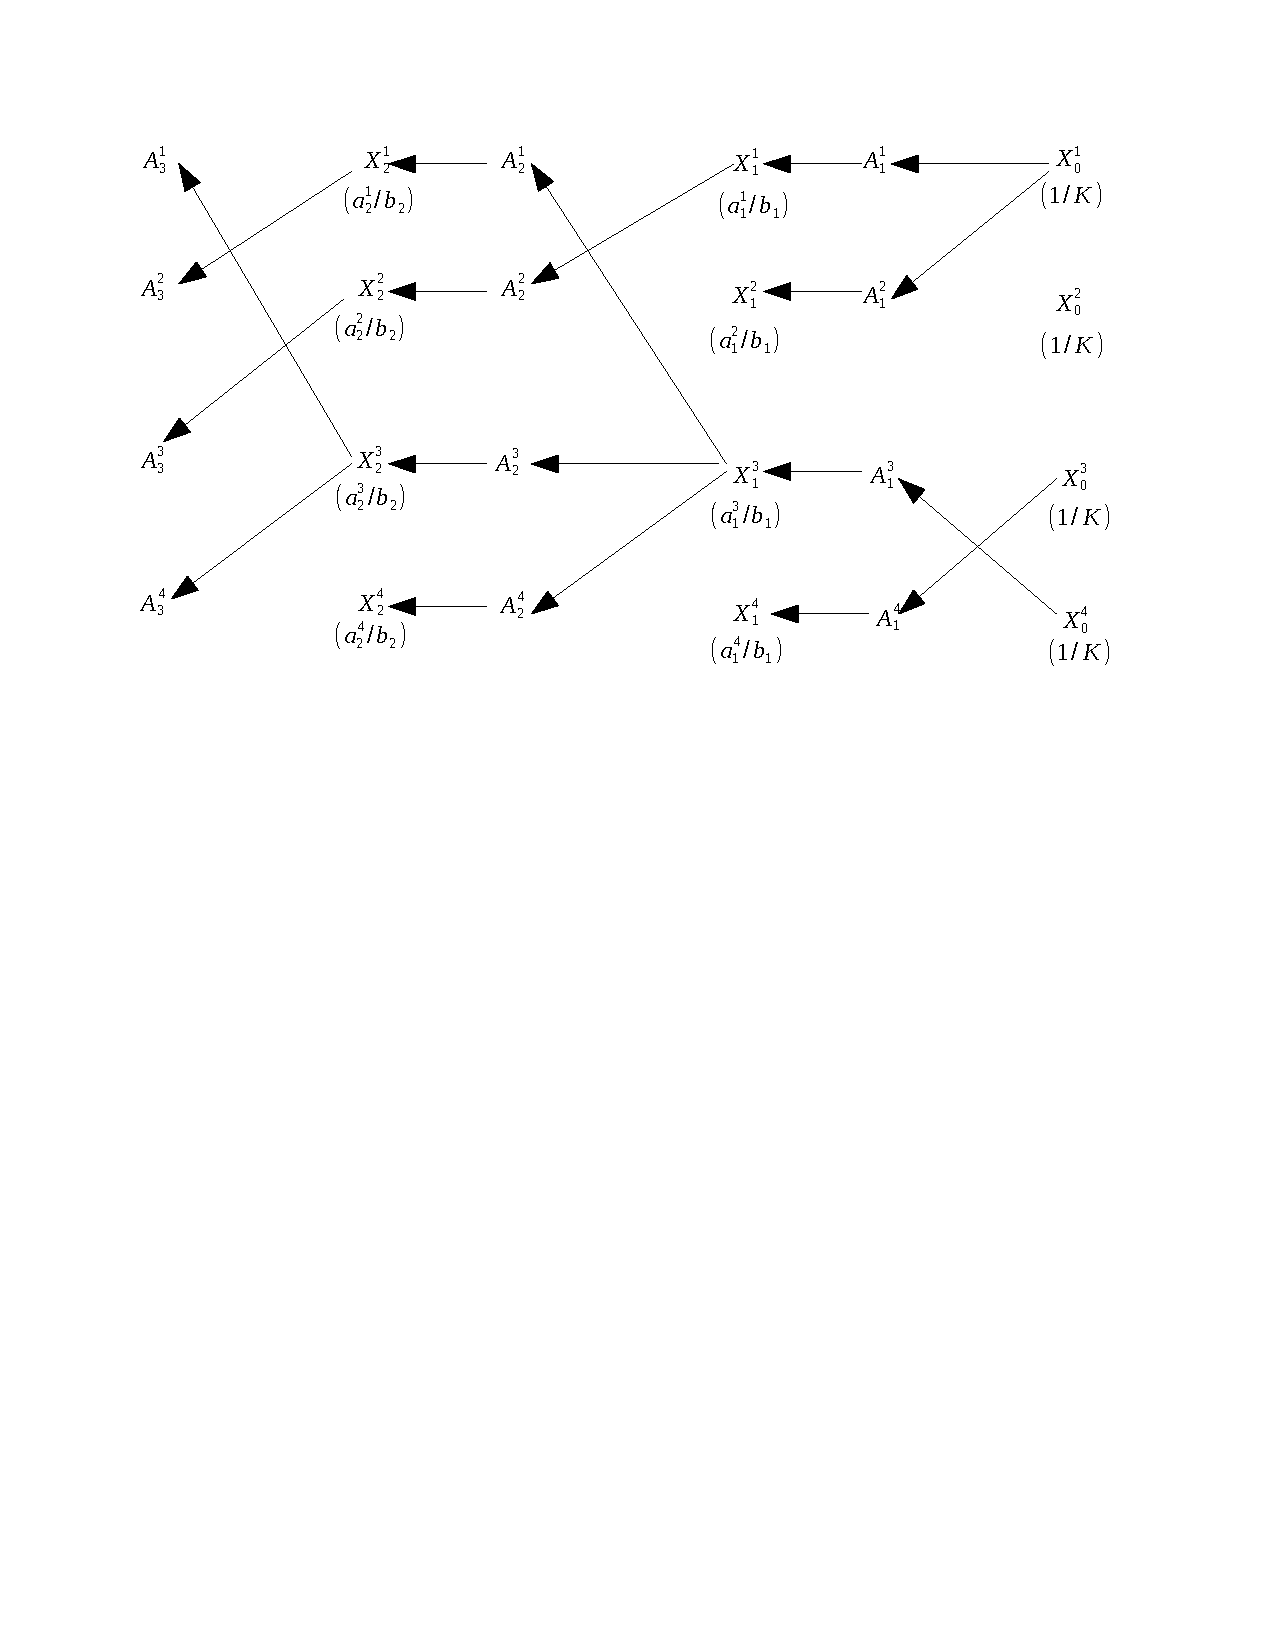
\includegraphics[width=\linewidth, trim=2cm 16cm 2.5cm 2cm, clip]{AnandsEstimator.pdf}
  \caption{A possible realization of the re-sampling procedure. $n =
    3$, $K = 4$. A number in a parenthesis indicates the probability
    of the unit vector above it being chosen to the next step.}
  \label{fig:AnandsEstimator}
\end{figure}
The difficulty with brute-force simulation and estimation is that,
when $n$ is large, the variance of $|A_n \cdots A_1 X_0|^\alpha$
is very large too, resulting in uselessly inaccurate estimations. One
approach of variance reduction is re-sampling. We divide the
estimation of $\Lambda(\alpha)$ into $n$ steps and we are prepared to
simulate $K$ realizations of $A_n, \dots, A_1$ and $X_0$. For
convenience, let
\begin{eqnarray*}
  M_n &=& A_n \cdots A_1 X_0 \\
  X_n &=& {M_n \over |M_n|}
\end{eqnarray*}
We can write
\begin{eqnarray*}
  M_n &=& A_n X_{n - 1} |M_{n - 1}| \\
  &=& A_n X_{n - 1} |A_{n-1} X_{n-2}| \cdot |M_{n-2}| \\
  &=& \cdots \\
  |M_n|^\alpha &=& \prod_{i=1}^n |A_i X_{i-1}|^\alpha
\end{eqnarray*}
With $K$ realizations of $A_n, \dots, A_1$ and $X_0$, a brute-force
estimator of ${1 \over n} \ln(\E |M_n|^\alpha)$ can be
\[
{1 \over n} \ln \left(
  {1 \over K} \sum_{l=1}^K \prod_{i=1}^n |A_i^l X^l_{i-1}|^\alpha
\right)
\]
where $A_i^l$ denotes the $l$-th realization of $A_i$ and
$X^l_{i-1} = A_{i-1}^l X^l_{i-2}/|A_{i-1}^l X^l_{i-2}|$. To reduce the
variance of the estimator, we introduce a re-sampling procedure:
\begin{equation}
  \label{eq:AnandsEstimator}
  \mathscr E_\alpha =
  {1 \over n}
  \sum_{i=1}^n \ln \left(
    {1 \over K}\sum_{l=1}^K |A_i^l X^{w_{l, i-1}}_{i-1}|^\alpha
  \right)
\end{equation}
where the random variable $w_{l, i-1}$ has conditional distribution
\begin{eqnarray*}
  \P(w_{l, i-1} = j | w_{1, i-2}, \dots, w_{K, i-2}) &=& {a^j_{i-1} \over b_{i-1}} \\
  a_{i-1}^j &=& |A_{i-1}^j X_{i-2}^{w_{j, i-2}}|^\alpha \\
  b_{i-1} &=& \sum_{l=1}^K a_{i-1}^l
\end{eqnarray*}
\begin{theorem}
  \[
  \E \left\{
    \sum_{i=1}^n \ln \left(
      {1 \over K}\sum_{l=1}^K |A_i^l X^{w_{l, i-1}}_{i-1}|^\alpha
    \right)
  \right\} = \ln \left(
    \E |A_n \cdots A_1 X_0|^\alpha
  \right)
  \]
\end{theorem}
Figure \ref{fig:AnandsEstimator} shows a possible realization of the
resampling procedure and algorithm \ref{alg:Lambda_estimation}
outlines an implementation of $\mathscr E_\alpha$. We take
$|\cdot|$ as the max norm.
For an GARCH(p, q) processes, the $A_i$ matrices have dimension
$d \times d$, where $d = p + q - 1$, and the $X_i$ are $d$-dimensional
unit vectors. 
\begin{algorithm}[H]
  \caption{Algorithm for estimating
    $\Lambda(\alpha) = \lim_{n \to \infty} {1 \over n} \ln\left(\E |A_n \cdots A_1|^\alpha \right)$}
  \label{alg:Lambda_estimation}
  \begin{algorithmic}
    \Procedure{$\mathscr E_\alpha$}{$n, K$}
    \State Define $K$ $d$-dimensional vectors $X^1, \dots, X^K$
    \State Define $K$ $d$-dimensional vectors $Y^1, \dots, Y^K$
    \State Define $K$-dimensional vector $a \gets (1, 1, \dots, 1)$
    \Comment{Initialize the weights}
    \For {$i$ from 1 to $K$}\Comment{Generate initial unit vectors}
    \For {$k$ from 1 to $d$}
    \State Generate a $U(0, 1)$ variable $U$
    \State $X^i(k) \gets U$ \Comment{$X^i(k)$ is the $k$-th component of $X^i$}
    \EndFor
    \State $X^i \gets X^i/|X^i|$
    \EndFor

    $\Lambda \gets 0$

    \For{$j$ from 1 to $n$}

    \State Define $K$-dimensional vector $Q$
    \State $Q(k) \gets \sum_{i=1}^k a(i)$ for all $k=1,2,\dots, K$
    \State Generate $K$ $d \times d$ random matrices $A^1, \dots, A^K$.

    \For{$k$ from 1 to $K$}
    \State Generate a $U(0, Q(K))$ variable $U$.
    \State $l \gets \min\{1 \leq i \leq K: Q(i) > U\}$
    \State $Y^k \gets A^k X^l$
    \State $a(k) \gets |Y^k|$
    \State $Y^k \gets Y^k/a(k)$
    \State $a(k) \gets a(k)^\alpha$
    \EndFor

    \State For all $k=1,\dots,K$, $X^k \gets Y^k$
    \State $\Lambda \gets \Lambda + {1 \over n}\ln\left( { Q(K) \over K} \right)$
    \EndFor
    \State $\Lambda \gets \Lambda + {1 \over n}\ln\left[ {1 \over K}\sum_{k=1}^K a(k) \right]$

    \Return $\Lambda$
    \EndProcedure
  \end{algorithmic}
\end{algorithm}

\subsection{GARCH(2,1) process}
As examples of the algorithm described in the previous section, we
consider GARCH(2,1) processes. In this particular case we have
\begin{eqnarray*}
  \sigma_t^2 &=& \omega + \alpha_1 R_{t-1}^2 + \alpha_2 R_{t-2}^2 +
  \beta_1 \sigma_{t-1}^2
\end{eqnarray*}
Or in matrix forms
\begin{eqnarray*}
  \begin{pmatrix}
    \sigma_t^2 \\
    R_{t-1}^2
  \end{pmatrix}
  &=&
  \begin{pmatrix}
  \alpha_1 Z_{t-1}^2 + \beta_1 & \alpha_2 \\
  Z_{t-1}^2 & 0
  \end{pmatrix}
  \begin{pmatrix}
    \sigma_{t-1}^2 \\
    R_{t-2}^2
  \end{pmatrix}
  +
  \begin{pmatrix}
    \omega \\
    0
  \end{pmatrix}
\end{eqnarray*}
where $R_t$ is the $t$-th observation of the sequence in question and
$Z_t$ are i.i.d $N(0,1)$ random variables. To estimate the 
values of $\omega, \alpha_1, \alpha_2, \beta_1$, we use the ``fGarch''
package of the ``R'' language. Its ``garchFit'' function provides
routine to fit a specified type of model to a given series.
The ``garchFit'' function provides 4 algorithms for maximum likelihood
estimation of the parameters. We choose its default algorithm ``nlminb'',
i.e. ``unconstrained and box-constrained optimization using PORT
routines''. The ``fGarch'' package is developed and maintained by {\it
Rmetrics} (https://www.rmetrics.org/).

  
\subsubsection{S\&P 500}
\begin{itemize}
\item GARCH(1, 1)
  When modeled as a GARCH(1, 1) process, the S\&P 500 return series
  has the coefficients as shown in the following equation
  \[
  \sigma_t^2 = 0.15 R_{t-1}^2 + 0.72 \sigma_{t-1}^2 + 7.4 \times 10^{-6}
  \]
  The tail index of the stationary distribution of $\sigma_t^2$ is
  estimated at 4.4465. On the other hand, the Hill estimator puts the
  tail index of the inferred $\sigma_t^2$ at 4.3372.

\item GARCH(2, 1)
  When fitted to a GARCH(2, 1) process, the S\&P 500 return series has
  the following model
  %% 7.949678e-02, 8.765884e-02, 9.376992e-06
  \[
  \sigma_t^2 = 0.079 R_{t-1}^2 + 0.088 R_{t-2}^2 + 0.668 \sigma_{t-1}^2 + 9.4 \times 10^{-6}
  \]
  Using the proposed re-sampling algorithm, our estimate of the tail
  index is $4.30026$. The values of $\Lambda(\alpha)$ in the
  neighborhood of $\alpha = \xi$ is listed in table
  \ref{tab:SP500_garch21_tail_index}.
  \begin{table}[htb!]
    \centering
    \begin{tabular}{l|l|l|l||l|l|l|l}
      $\alpha$ & $\Lambda(\alpha)$ & err. & rel. err. & $\alpha$ & $\Lambda(\alpha)$ & err. & rel. err. \\
      \hline
      0.1000 & -0.0186 & 0.0007 & 0.0378 & 3.1000 & -0.2020 & 0.2175 & 1.0766\\
      0.2000 & -0.0366 & 0.0012 & 0.0329 & 3.2000 & -0.1921 & 0.2360 & 1.2286\\
      0.3000 & -0.0539 & 0.0016 & 0.0293 & 3.3000 & -0.1829 & 0.2765 & 1.5116\\
      0.4000 & -0.0706 & 0.0020 & 0.0281 & 3.4000 & -0.1705 & 0.3121 & 1.8308\\
      0.5000 & -0.0866 & 0.0024 & 0.0279 & 3.5000 & -0.1595 & 0.3335 & 2.0914\\
      0.6000 & -0.1018 & 0.0030 & 0.0299 & 3.6000 & -0.1458 & 0.3665 & 2.5140\\
      0.7000 & -0.1163 & 0.0045 & 0.0387 & 3.7000 & -0.1264 & 0.4249 & 3.3627\\
      0.8000 & -0.1301 & 0.0059 & 0.0456 & 3.8000 & -0.1165 & 0.4285 & 3.6778\\
      0.9000 & -0.1432 & 0.0083 & 0.0581 & 3.9000 & -0.0996 & 0.5233 & 5.2545\\
      1.0000 & -0.1552 & 0.0104 & 0.0668 & 4.0000 & -0.0819 & 0.5479 & 6.6896\\
      1.1000 & -0.1666 & 0.0137 & 0.0825 & 4.1000 & -0.0653 & 0.5806 & 8.8930\\
      1.2000 & -0.1771 & 0.0168 & 0.0947 & 4.2000 & -0.0403 & 0.7173 & 17.8196\\
      1.3000 & -0.1867 & 0.0206 & 0.1105 & 4.3000 & -0.0365 & 0.6749 & 18.5091\\
      1.4000 & -0.1958 & 0.0246 & 0.1255 & 4.4000 & -0.0055 & 0.7390 & 135.2172\\
      1.5000 & -0.2038 & 0.0299 & 0.1467 & 4.5000 & 0.0186 & 0.8443 & 45.4573\\
      1.6000 & -0.2107 & 0.0353 & 0.1675 & 4.6000 & 0.0267 & 0.7493 & 28.0286\\
      1.7000 & -0.2169 & 0.0398 & 0.1836 & 4.7000 & 0.0614 & 0.9068 & 14.7576\\
      1.8000 & -0.2226 & 0.0467 & 0.2099 & 4.8000 & 0.0867 & 0.9380 & 10.8220\\
      1.9000 & -0.2271 & 0.0543 & 0.2392 & 4.9000 & 0.0973 & 0.8703 & 8.9467\\
      2.0000 & -0.2299 & 0.0607 & 0.2642 & 5.0000 & 0.1275 & 0.9424 & 7.3918\\
      2.1000 & -0.2320 & 0.0685 & 0.2953 & 5.1000 & 0.1618 & 1.0582 & 6.5403\\
      2.2000 & -0.2344 & 0.0760 & 0.3244 & 5.2000 & 0.1721 & 0.8950 & 5.2004\\
      2.3000 & -0.2343 & 0.0903 & 0.3856 & 5.3000 & 0.2081 & 0.9849 & 4.7334\\
      2.4000 & -0.2341 & 0.0994 & 0.4246 & 5.4000 & 0.2411 & 1.0852 & 4.5009\\
      2.5000 & -0.2320 & 0.1106 & 0.4767 & 5.5000 & 0.2378 & 0.9362 & 3.9375\\
      2.6000 & -0.2291 & 0.1273 & 0.5555 & 5.6000 & 0.2605 & 0.9805 & 3.7635\\
      2.7000 & -0.2273 & 0.1365 & 0.6007 & 5.7000 & 0.3306 & 1.0445 & 3.1596\\
      2.8000 & -0.2214 & 0.1595 & 0.7205 & 5.8000 & 0.3301 & 1.0014 & 3.0333\\
      2.9000 & -0.2143 & 0.1667 & 0.7781 & 5.9000 & 0.3562 & 1.0427 & 2.9270\\
      3.0000 & -0.2075 & 0.2034 & 0.9804 & 6.0000 & 0.3891 & 0.9544 & 2.4525
    \end{tabular}
    \caption{SP500: $\Lambda(\alpha)$ around $\alpha = \xi$. N = 400, K = 40000}
    \label{tab:SP500_garch21_tail_index}
  \end{table}

  \begin{minipage}{0.5\linewidth}
    \centering
    $\Lambda(\alpha)$
    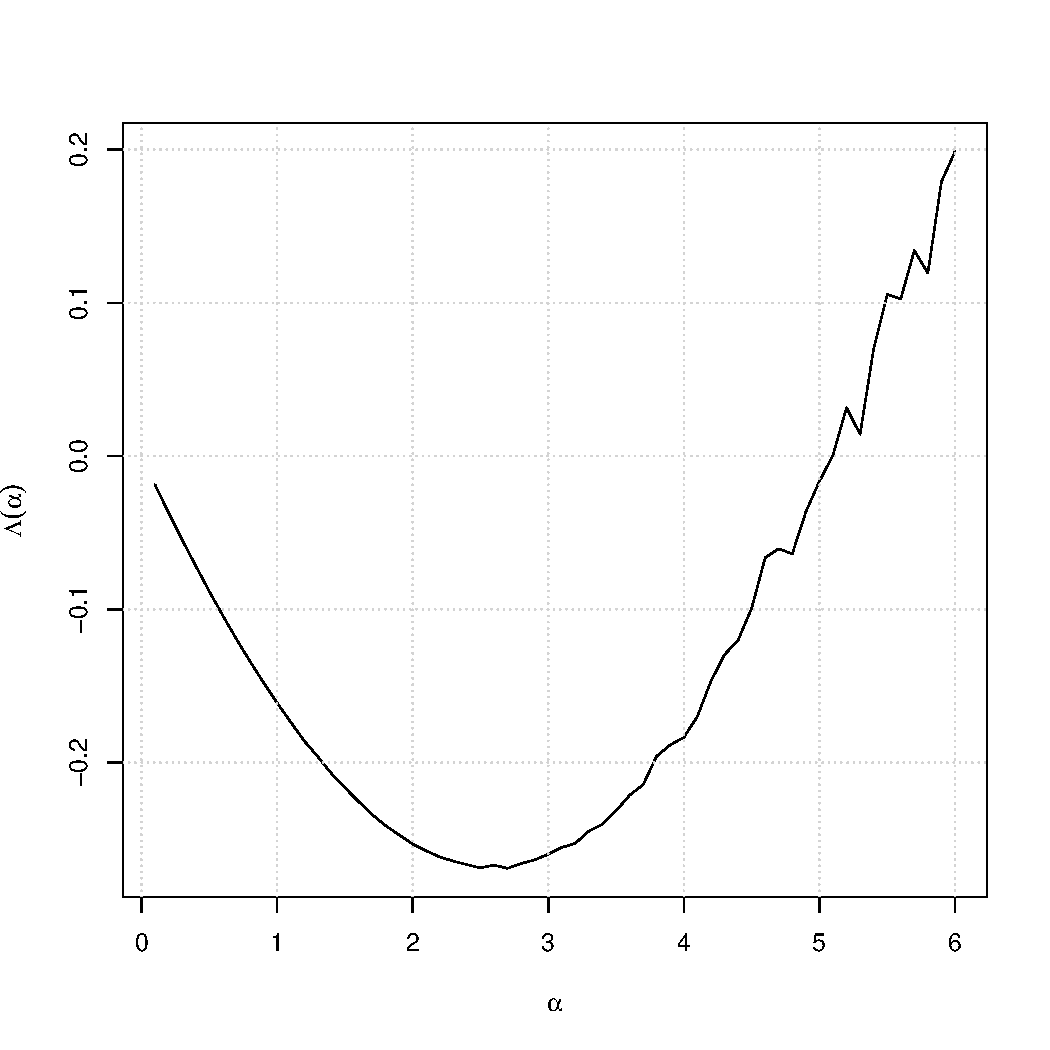
\includegraphics[width=\textwidth]{SP500_xi.pdf}
  \end{minipage}\hfill
  \begin{minipage}{0.5\linewidth}
    \centering
    $r_\xi(x)$ corresponding to $\xi$
    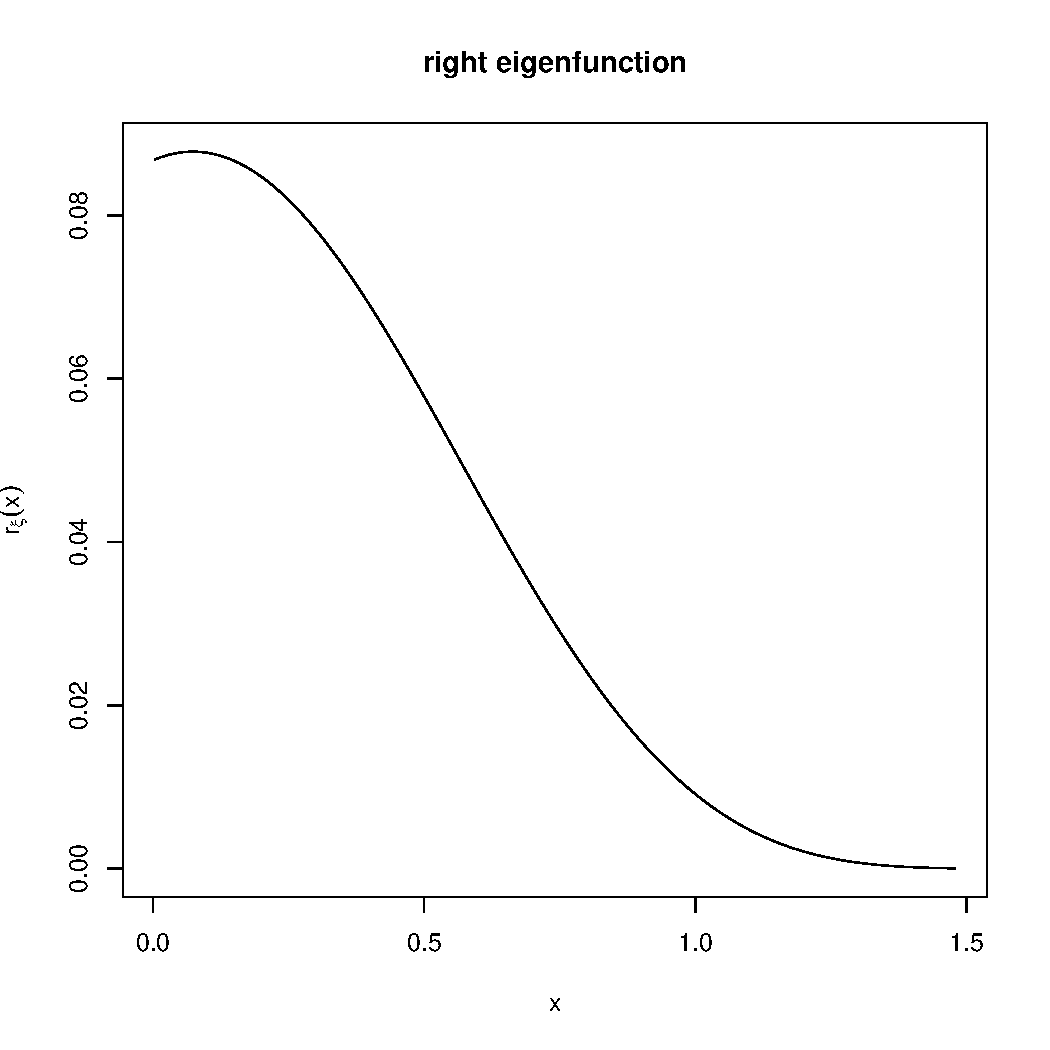
\includegraphics[width=\textwidth]{SP500_r.pdf}
  \end{minipage}
  
  
\end{itemize}

\subsubsection{DAX}
\begin{itemize}
\item GARCH(1, 1)
  When modeled as a GARCH(1, 1) process, the DAX return series
  has the coefficients as shown in the following equation
  \[
  \sigma_t^2 = 0.06 R_{t-1}^2 + 0.92 \sigma_{t-1}^2 + 3.1 \times 10^{-6}
  \]
  The tail index of the stationary distribution of $\sigma_t^2$ is
  estimated at 6.4269. The Hill estimator of this
  sequence is computed at 6.6020.
  % as the Hill plot in figure
  % \ref{fig:DAX_var_HillPlot} suggests.
  % \begin{figure}[htb!]
  %   \centering
  %   \includegraphics[scale=0.4]{DAX_var_HillPlot.pdf}    
  %   \caption{DAX $\sigma_t^2$ Hill Plot}
  %   \label{fig:DAX_var_HillPlot}
  % \end{figure}

\item GARCH(2, 1)
  When fitted to a GARCH(2, 1) process, the DAX return series has the following model
  \[
  \sigma_t^2 = 0.027 R_{t-1}^2 + 0.042 R_{t-2}^2 + 0.897 \sigma_{t-1}^2 + 4.0 \times 10^{-6}
  \]
  The algorithm with its current implementation has difficulty to
  estimate $\Lambda(\alpha)$ as $\alpha$ becomes large. This is shown
  in the figure below:
  \begin{figure}[htb!]
    \centering
    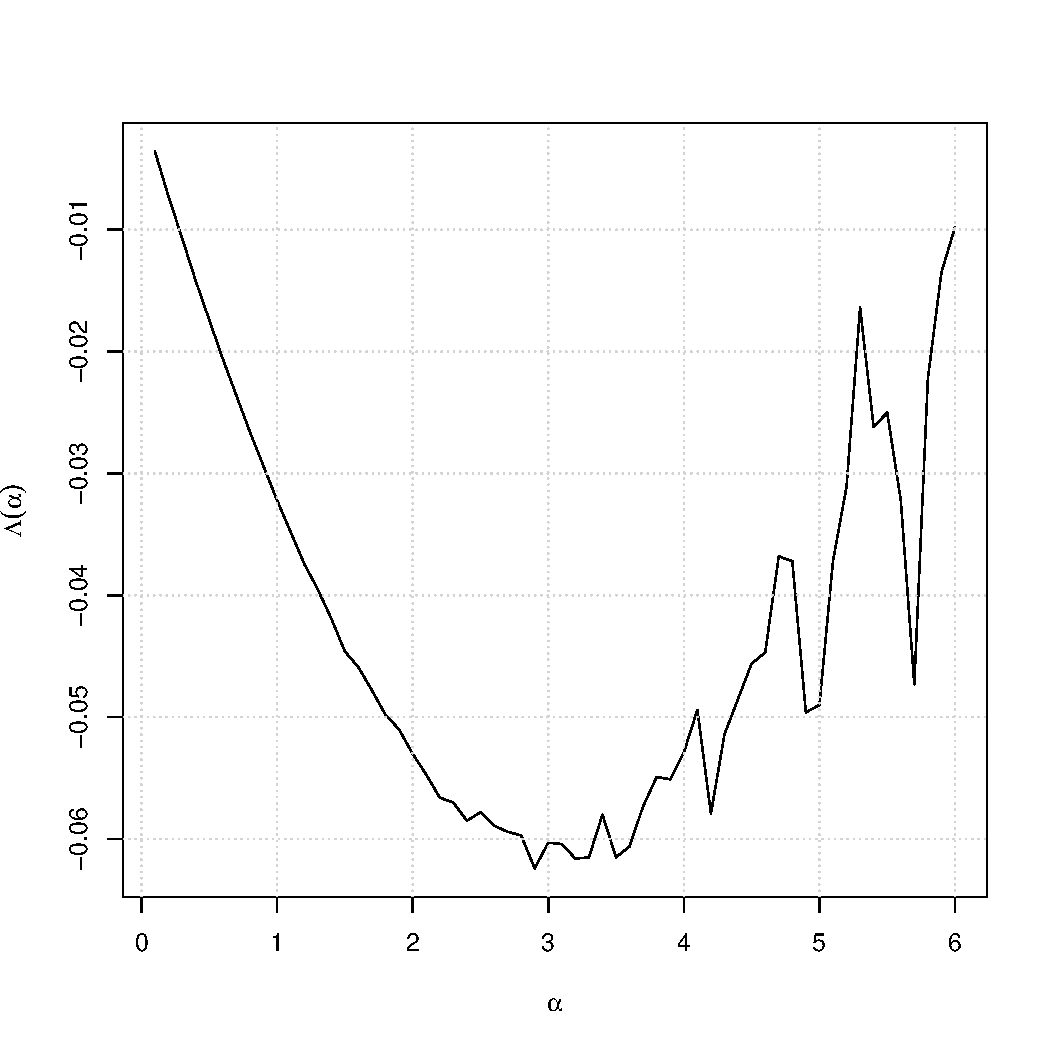
\includegraphics[width=\textwidth]{DAX_xi.pdf}
    \caption{$\Lambda(\alpha)$ estimates for DAX}
    \label{fig:DAX_garch21_tailindex}
  \end{figure}
  The estimated values of $\Lambda(\alpha)$ are listed table \ref{tab:DAX_garch21_tail_index}.
    \begin{table}[htb!]
    \centering
    \begin{tabular}{l|l|l|l||l|l|l|l}
      $\alpha$ & $\Lambda(\alpha)$ & err. & rel. err. & $\alpha$ & $\Lambda(\alpha)$ & err. & rel. err. \\
      \hline
      0.1000 & -0.0036 & 0.0009 & 0.2535 & 3.1000 & -0.0604 & 0.2027 & 3.3558 \\
      0.2000 & -0.0073 & 0.0017 & 0.2340 & 3.2000 & -0.0616 & 0.2585 & 4.1940 \\
      0.3000 & -0.0107 & 0.0020 & 0.1903 & 3.3000 & -0.0615 & 0.2669 & 4.3419 \\
      0.4000 & -0.0142 & 0.0025 & 0.1763 & 3.4000 & -0.0580 & 0.3232 & 5.5729 \\
      0.5000 & -0.0174 & 0.0027 & 0.1531 & 3.5000 & -0.0615 & 0.3719 & 6.0467 \\
      0.6000 & -0.0206 & 0.0030 & 0.1445 & 3.6000 & -0.0606 & 0.3794 & 6.2604 \\
      0.7000 & -0.0236 & 0.0038 & 0.1624 & 3.7000 & -0.0573 & 0.4485 & 7.8213 \\
      0.8000 & -0.0266 & 0.0050 & 0.1884 & 3.8000 & -0.0549 & 0.5345 & 9.7438 \\
      0.9000 & -0.0294 & 0.0073 & 0.2469 & 3.9000 & -0.0551 & 0.5655 & 10.2685 \\
      1.0000 & -0.0322 & 0.0089 & 0.2774 & 4.0000 & -0.0529 & 0.6865 & 12.9826 \\
      1.1000 & -0.0348 & 0.0109 & 0.3127 & 4.1000 & -0.0494 & 0.7077 & 14.3304 \\
      1.2000 & -0.0374 & 0.0146 & 0.3904 & 4.2000 & -0.0579 & 0.7418 & 12.8088 \\
      1.3000 & -0.0395 & 0.0178 & 0.4515 & 4.3000 & -0.0514 & 0.8021 & 15.6075 \\
      1.4000 & -0.0419 & 0.0218 & 0.5210 & 4.4000 & -0.0485 & 0.9369 & 19.3079 \\
      1.5000 & -0.0446 & 0.0260 & 0.5821 & 4.5000 & -0.0456 & 0.9525 & 20.8980 \\
      1.6000 & -0.0459 & 0.0304 & 0.6634 & 4.6000 & -0.0447 & 1.0402 & 23.2610 \\
      1.7000 & -0.0478 & 0.0356 & 0.7443 & 4.7000 & -0.0368 & 1.0678 & 28.9796 \\
      1.8000 & -0.0498 & 0.0421 & 0.8452 & 4.8000 & -0.0372 & 1.1068 & 29.7502 \\
      1.9000 & -0.0510 & 0.0482 & 0.9443 & 4.9000 & -0.0496 & 1.1848 & 23.8698 \\
      2.0000 & -0.0530 & 0.0543 & 1.0236 & 5.0000 & -0.0490 & 1.1304 & 23.0528 \\
      2.1000 & -0.0547 & 0.0650 & 1.1877 & 5.1000 & -0.0372 & 1.3674 & 36.7623 \\
      2.2000 & -0.0566 & 0.0713 & 1.2610 & 5.2000 & -0.0311 & 1.3533 & 43.5658 \\
      2.3000 & -0.0570 & 0.0820 & 1.4393 & 5.3000 & -0.0164 & 1.3191 & 80.2003 \\
      2.4000 & -0.0585 & 0.0914 & 1.5631 & 5.4000 & -0.0262 & 1.4752 & 56.2897 \\
      2.5000 & -0.0578 & 0.1070 & 1.8514 & 5.5000 & -0.0250 & 1.3379 & 53.5797 \\
      2.6000 & -0.0589 & 0.1163 & 1.9759 & 5.6000 & -0.0322 & 1.4219 & 44.1810 \\
      2.7000 & -0.0594 & 0.1302 & 2.1913 & 5.7000 & -0.0473 & 1.3915 & 29.4468 \\
      2.8000 & -0.0597 & 0.1516 & 2.5405 & 5.8000 & -0.0222 & 1.6773 & 75.3996 \\
      2.9000 & -0.0624 & 0.1663 & 2.6664 & 5.9000 & -0.0135 & 1.4893 & 110.0806 \\
      3.0000 & -0.0603 & 0.1877 & 3.1148 & 6.0000 & -0.0098 & 1.5522 & 158.6270
    \end{tabular}
    \caption{DAX: $\Lambda(\alpha)$ around $\alpha = \xi$. N = 400, K = 40000}
    \label{tab:DAX_garch21_tail_index}
  \end{table}


  %% \begin{minipage}{0.5\linewidth}
  %%   \centering
  %%   $\Lambda(\alpha)$
  %%   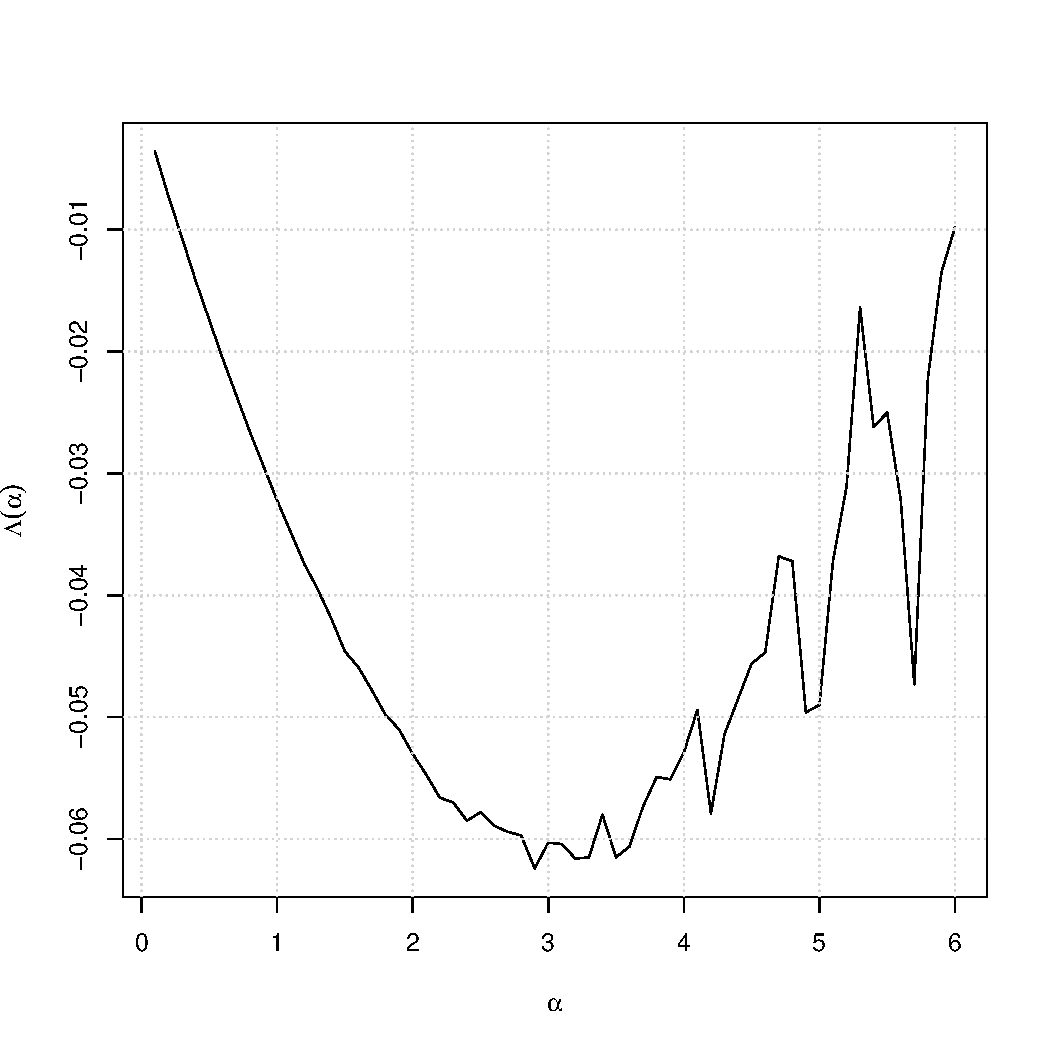
\includegraphics[width=\textwidth]{DAX_xi.pdf}
  %% \end{minipage}\hfill
  %% \begin{minipage}{0.5\linewidth}
  %%   \centering
  %%   $r_\xi(x)$ corresponding to $\xi$
  %%   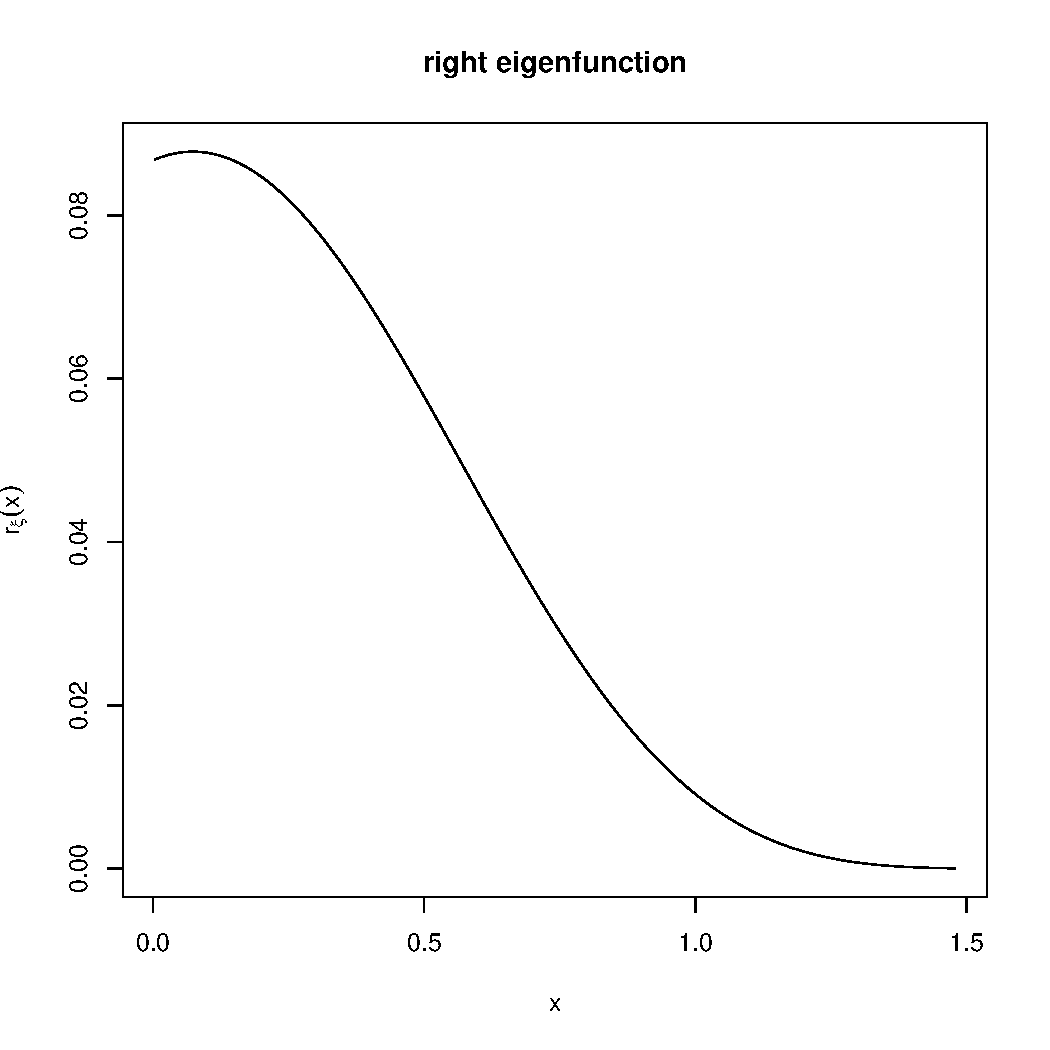
\includegraphics[width=\textwidth]{SP500_r.pdf}
  %% \end{minipage}

  % \begin{table}[htb!]
  %   \centering
  %   \begin{tabular}{c|c|c|c}
  %     $\alpha$ & $\Lambda(\alpha)$ & abs. err. & rel. err. \\
  %     \hline
  %     0.1000 & -0.0017 & 0.0026 & 1.5402 \\
  %     0.2000 &  0.0009 & 0.0053 & 6.1829 \\
  %     0.3000 &  0.0077 & 0.0075 & 0.9712 \\
  %     0.4000 &  0.0192 & 0.0096 & 0.4975 \\
  %     0.5000 &  0.0355 & 0.0121 & 0.3411 \\
  %   \end{tabular}
  %   \caption{$\Lambda(\alpha)$ of DAX as GARCH(2,1)}
  %   \label{tab:DAX_garch21_Lambda}
  % \end{table}
  % The tail index is estimated at 0.1801.
\end{itemize}

\section{Evaluation of the right eigenfunction}

\section*{Acknowledgements}

% \begin{supplement}
% \sname{Supplement A}\label{suppA}
% \stitle{Title of the Supplement A}
% \slink[url]{http://www.e-publications.org/ims/support/dowload/imsart-ims.zip}
% \sdescription{Dum esset rex in
% accubitu suo, nardus mea dedit odorem suavitatis. Quoniam confortavit
% seras portarum tuarum, benedixit filiis tuis in te. Qui posuit fines tuos}
% \end{supplement}


% \begin{thebibliography}{9}

% \bibitem{r1}
% \textsc{Billingsley, P.} (1999). \textit{Convergence of
% Probability Measures}, 2nd ed.
% Wiley, New York.
% \MR{1700749}


% \bibitem{r2}
% \textsc{Bourbaki, N.}  (1966). \textit{General Topology}  \textbf{1}.
% Addison--Wesley, Reading, MA.

% \bibitem{r3}
% \textsc{Ethier, S. N.} and \textsc{Kurtz, T. G.} (1985).
% \textit{Markov Processes: Characterization and Convergence}.
% Wiley, New York.
% \MR{838085}

% \bibitem{r4}
% \textsc{Prokhorov, Yu.} (1956).
% Convergence of random processes and limit theorems in probability
% theory. \textit{Theory  Probab.  Appl.}
% \textbf{1} 157--214.
% \MR{84896}

% \end{thebibliography}

\bibliographystyle{unsrt}
\bibliography{../../thesis/econophysics}
\end{document}
